\documentclass{article}
\usepackage[margin = 1 in]{geometry}
\usepackage{amsfonts, amsmath, amssymb}
\usepackage[none]{hyphenat}
\usepackage{fancyhdr}
\usepackage{listings}
\usepackage[nottoc,notlot,notlof]{tocbibind}
\usepackage{amsmath}  % for \text macro
\usepackage{amssymb}  % for \mathbb macro
\usepackage{graphicx}
\usepackage[spaces,hyphens]{url}
\usepackage[utf8]{inputenc}


\newtheorem{theorem}{Theorem}
\newenvironment{proof}{\noindent{\bf Proof:}}{$\hfill \Box$ \vspace{10pt}}  
\pagestyle{fancy}
\fancyhead{}
\fancyfoot{}
\fancyhead[L]{\slshape \MakeUppercase{3D AutoGeneration}}
\fancyhead[R]{\slshape Feasibility Report}
\fancyhead[C]{\thepage}
\renewcommand{\footrulewidth}{0pt}
\parindent 0ex
\setlength{\parindent}{4em}
\setlength{\parskip}{1em}
\renewcommand{\baselinestretch}{1.5}
\begin{document}
\begin{titlepage}
\begin{center}
\vspace*{1cm}
\begin{figure}[h!]
\centering

\includegraphics[scale=0.5]{logo}
\end{figure}
\Large\textbf{Feasibility Report}\\
\Large\textbf{Final Year Project}\\
\vfill
\line(1,0){400}\\[1mm]
\huge{\textbf{Auto Generation of 3D model from room images}}\\[3mm]
\line(1,0){400}\\
\vfill
\large{\textbf{Tooba Naseer  (2016-CE-72)}}\\
\large{\textbf{Rida Mahmood  (2016-CE-54)}}\\
\large{\textbf{Ayesha Jabbar  (2016-CS-159)}}\\
\large{\textbf{Rabeya Hamood  (2016-CE-81)}}\\
\large{\textbf{Supervised by: Dr. Sheikh Faisal Rasheed}}\\
\large{\textbf{Department of Computer Science and Engineering}}\\
\large{\textbf{University of Engineering and Technology, Lahore}}\\
\end{center}
\end{titlepage}
\tableofcontents
\thispagestyle{empty}
\clearpage
\setcounter{page}{1}

\makeatletter
\newcommand{\heading}[1]% #1 = text
{\par\vskip 1.5ex \@plus .2ex
 \hangindent=1em
 \noindent\makebox[1em][l]{$\,\bullet$}\textbf{\large #1}%
\par\vskip 1.5ex \@plus .2ex
\@afterheading}
\makeatother

\section{Introduction}

\subsection{Overview of Project}
In the world full of wishes, everyone wants his house according to his own wish but he don't know how his house will look after proper adjustment of furniture and floor texture in the real environment inside the rooms. He cannot only rely on architects or house-map designers to make his house map or plan. Moreover, the ever growing world of 3D technologies fascinating the users and home planners to create and edit 3D models randomly using specified textures and furniture given in a certain application.
\\
\\
This project intent to the auto-generation of 3D models from 2D imported floor plans. It can be operated by importing a 2D floor plan in an image format. The techniques of image processing and model mapping used to generate the 3D computer graphics model according to the imported 2D floor plan. The 3D modification function provides ability to change the texture of floor and walls; moreover, it also enables users to add furniture in 3D constructed model. User can look at 3D model from different viewpoints i.e. top-view, walk-through, front-view and side-view.
\subsection{Background}
There has been a great incentive in generating 3D models from images of 2D floor plans using image processing\cite{ImageP} and computer graphics techniques. Our research scope embeds to those areas of interests who generate 3D models by taking floor plan in different formats or use special tools  to sketch 2D floor plan on a special editor. Some lead their research in the area of computer vision to generate models from images.
\\
\\
A scholar named Matthew Chandler research focuses on the automation of manual processes like wall extrusion, object mapping, floor and ceiling reconstruction\cite{abc}.In existing systems these processes are not automatic. So, in our our system we generate 3D model automatically i.e. on just button click.
Exiting systems like SketchUp can generate 3D models but they require a lot of manual task to perform after importing floor plan. Moreover, SweetHome3D make 3D models by drawing 2D floor plan on the editor which is quite hard for a nonprofessional user. So, how to get rid of much effort in generating 3D models according to your own wish?
Our project provides house planners, architects and common users to make 3D models automatically by just importing a 2D floor plan in an image format.
\subsection{Motivation}
A common user who does not know how their home look after construction and proper adjustment of their accessories, it’s a big platform for them to see their house in 3D more than their imagination. We move towards this project because many artists, civil constructors and common house owners which want houses according to their own designs, so to help them that their floor plan will look good or not after implementation, we are making this software. Already existing such systems can only used by technical users because a lot of manual work is required to construct 3D model from 2D file format. So, this motivates us to automatically generate 3D model from an imported 2D floor plan image by just clicking a button.\cite{research}\\
\section{Objectives of the project}
\subsection{Industry Objectives}
\begin{itemize}
\item Implement a system that takes into account the demands of industrial artists, home planners and architectural engineers when they designed 2D floor plans and want to see them in 3D before actual implementation.
\item To promote prospective and rapid development of a project by generating 3D models from 2D floor plans in just some moments. This leads to industrial workers save their time and cost.
\item To increase industry sales and profit by automatically generating 3D models which seeks customers attraction in less time. This system provides opportunity to estate builders and home-planners to grow market sales by investing less time and effort on their customers.
\item To grow market shares time by time because every planner wants to increase his share in this era of marketing. When most of the industrial house-planners want to use this proposed system, then they provide a large amount of 3D models of their 2D floor plans to the market, they will get profit over their sales and invest this profit to another venture. This will lead to grow their market shares.
\item To launch a new service which gives ability to view 3D models of 2D floor plans from different viewpoints. Planner can decide abruptly that which texture suits well to his house. It is also a way to increase customer attraction.
\end{itemize}
\subsection{Research Objectives}
\begin{itemize}
\item To apply automation for construction of 3D model via the successive collection of multi-sensorial data and research papers.
\item To analyze working different softwares which make 3D models via importing floor plans in different formats as input. So, we could research on existing softwares in market.
\item To verify, whether we are moving towards right technology and software in order to implement a 3D project.
\item To find out the planners/customers relationship on the behavior of house construction.
\item To identify the problems faced by users and planners while constructing houses according to their own 2D floor plan.
\item To provide the solution of the problems faced by planners and comon users while constructing houses.
\item To predict the behavior of people who were already using these kinds of softwares by importing or drawing their own 2D floor plans.
\item To develop a system which provides users to make decisions at right time before they start constructing their houses.
\item To assess the traditions of people i.e. which type of texture and maps they mostly want.

\end{itemize}
\subsection{Academic Objectives}
\begin{itemize}
\item	To ensure, that we are implementing our project by using latest technologies which helps students and technical persons to enhance their technical skills via learning.
\item Students will able to apply their knowledge and technical skills they have learned in these three years so far.

\end{itemize}
\section{Scope of the project}
In the autogeneration of 3D models, 3D tools and computer graphic techniques are used.
The scope of this project spread towards house planners, architects and common users
who want to make their houses according to their own wish.
This project handles files of 2D floor plans in image format (.png and .jpeg), then apply image
processing techniques on that floor plan to recognize objects and  generate a 3D model accordingly. 
Our application can be used by a common house owner or even by an architect.\cite{Projectscope}\\
\section{Target Audience}

\heading{Common Users}	
People of this era are full of wishes, they want their own designs to construct and adjust their houses.  Our software will enable common users to visualize 3D model according to their own choice of 2D floor plan. Avery easy to use GUI enables common users to do interior design of home.
\heading{Interior Designers} 
Our software helps interior designers in quick editing of 3D model without even wasting essential resources i.e. time and money.
\heading{Architects and Home planners} 
For architects or planners who are making floor plans for common people, this 3D software provides them ease and makes them to do less effort for customer satisfaction and increases the quality of  their service delivery in time. So, our software can also be used by architects and home planners.
\heading{Real estate sellers agents}
For people who are running real estate businesses, 3D floor plans could bring new ideas for efficient sales promotions. It could help them engage customers with interactive and informative site details of adjustment. So, our software can also be used by real estate agents.

\section{Possible Applications of work}
The system is related to the generation and modification of 3D model from 2D floor plan.
The possible applications of the system are:
\begin{itemize}
\item Importing of 2D floor plan in image format.



\begin{center}
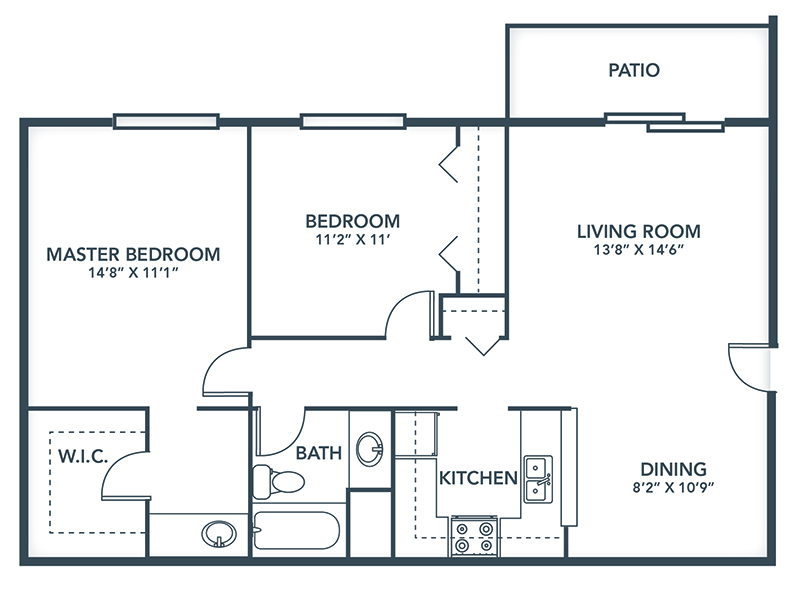
\includegraphics[scale=1]{floorplan}
\\Figure 1: 2D floor plan
\end{center}



\item Generate 3D model according to imported floor plan.


\begin{center}
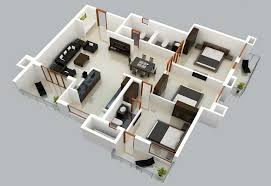
\includegraphics[scale=0.4]{3dmodel}
\\Figure 2: 3D generated model
\end{center}


\item Platform for interior designing of 3D generated model i.e.  Placement of furniture, changing of texture/paint color of walls and changing of floor designs.
\begin{center}
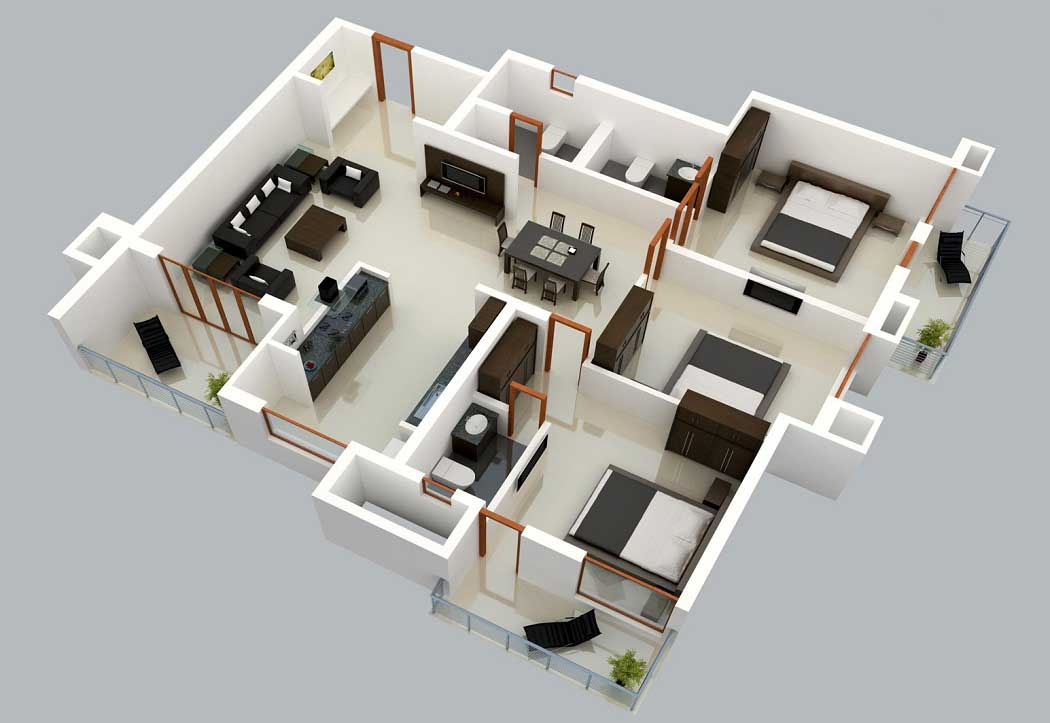
\includegraphics[scale=0.3]{3dhome}
\\Figure 3: 3D model interior designing
\end{center}
\item Platform for architects to generate 3D model efficiently with less time and effort.
\begin{center}
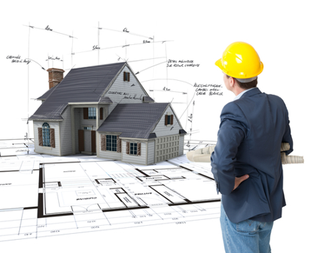
\includegraphics[scale=0.7]{architect}
\\Figure 4: Architects
\end{center}
\item Platform for home planners, real estate selling agents to win customer satisfaction and for efficient sales promotions.
\begin{center}
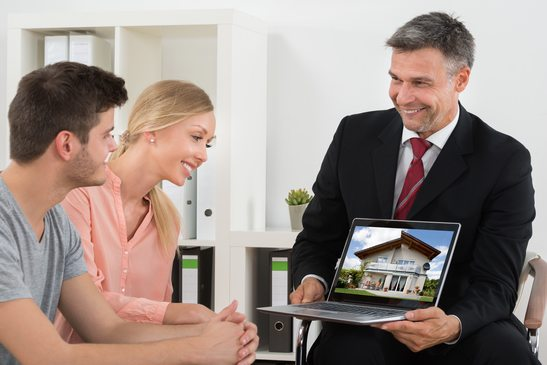
\includegraphics[scale=0.4]{real}
\\Figure 5: Interaction with customers
\end{center}
\end{itemize}
\section{Existing System}
\subsection{Comparison of Existing Systems}



\setlength{\arrayrulewidth}{1mm}
\setlength{\tabcolsep}{9pt}
\renewcommand{\arraystretch}{1.7}

\begin{tabular}{ |p{2cm}|p{4cm}|p{6cm}| }
\hline
\multicolumn{3}{|c|}{Comparison of Existing Systems} \\
\hline
Software&Developed By&Key Features\\
\hline
SketchUp&Brad Schell,Trimble Inc.&2D drawing, 3D Modelling, Panoramic 360 Views, Parrametric Model, Textures\\
\hline
SweetHome3D&Abcd &2D drawing, 3D Modelling, Panoramic 360 Views, Parrametric Model\\
\hline
Blender&Ton Roosendaal&Rendering, Game Creation,
Animation Toolset, Visual Effects.
\\
\hline
Free CAD Software&Jürgen Riegel, Werner Mayer, Yorik van Havre&2D drawing, 3D Modelling, Panoramic 360 Views, Parametric Model\\
\hline
SolidWorks&Autodesk&2D Drawing, 3D solid Modelling, 3D model editing\\
\hline
\end{tabular}

\heading{Further Comparison}
\begin{tabular}{|p{2cm}|p{2cm}|p{2cm}|p{4cm}|p{2cm}|p{2cm}|  }
\hline
\multicolumn{6}{|c|}{Comparison of Existing Systems} \\
\hline
Software&Type of Software&Platform Supported	&Backend-Technology	&Deployment	&Difficulty Level\\
\hline
SketchUp&Freemium&Windows and Mac&Written in C++ and Objective-C. Open GL is used as a display layer.&Open API(For In-process apps)&Average\\
\hline
SweetHome3d&Free and open source&Linux, Mac OS X, Solaris and Windows&Written in Java. Java3D is used for graphics.&Open API&Easy\\
\hline
Blender&Free and open source&Windows, MacOS, Linux, Free BSD, OpenBSD&Written in C and there is tiny bit of Python for API and included scripts. It uses OpenGL, a graphics API.	&Open API&Difficult\\
\hline
FreeCAD Software&Free and open source& MacOS, Unix, Windows&Written in C++, Python. The interface is built with Qt. &Open API&Average\\
\hline
SolidWorks&Only Free trial version is available&Windows, MacOS&Written in C++	&Open API&Difficult\\
\hline
\end{tabular}






\subsection{Drawbacks of Existing Systems}
\heading{SketchUp}
SketchUp is commonly used by architects, civil engineers and mechanical engineers for the purpose of architectural design. This software mainly focuses on the design of architectural building ad less focus on interior design. So this software is not suitable for interior design. This software cannot generate 3D model automatically. It required a lot of manual work in creating 3D model. For example before generating 3D model, users must trace the floor plan image and then extrude the walls by using SketchUp provided tools. So, it is not easy to use for non-technical users.\cite{sketchup}\\
\begin{center}
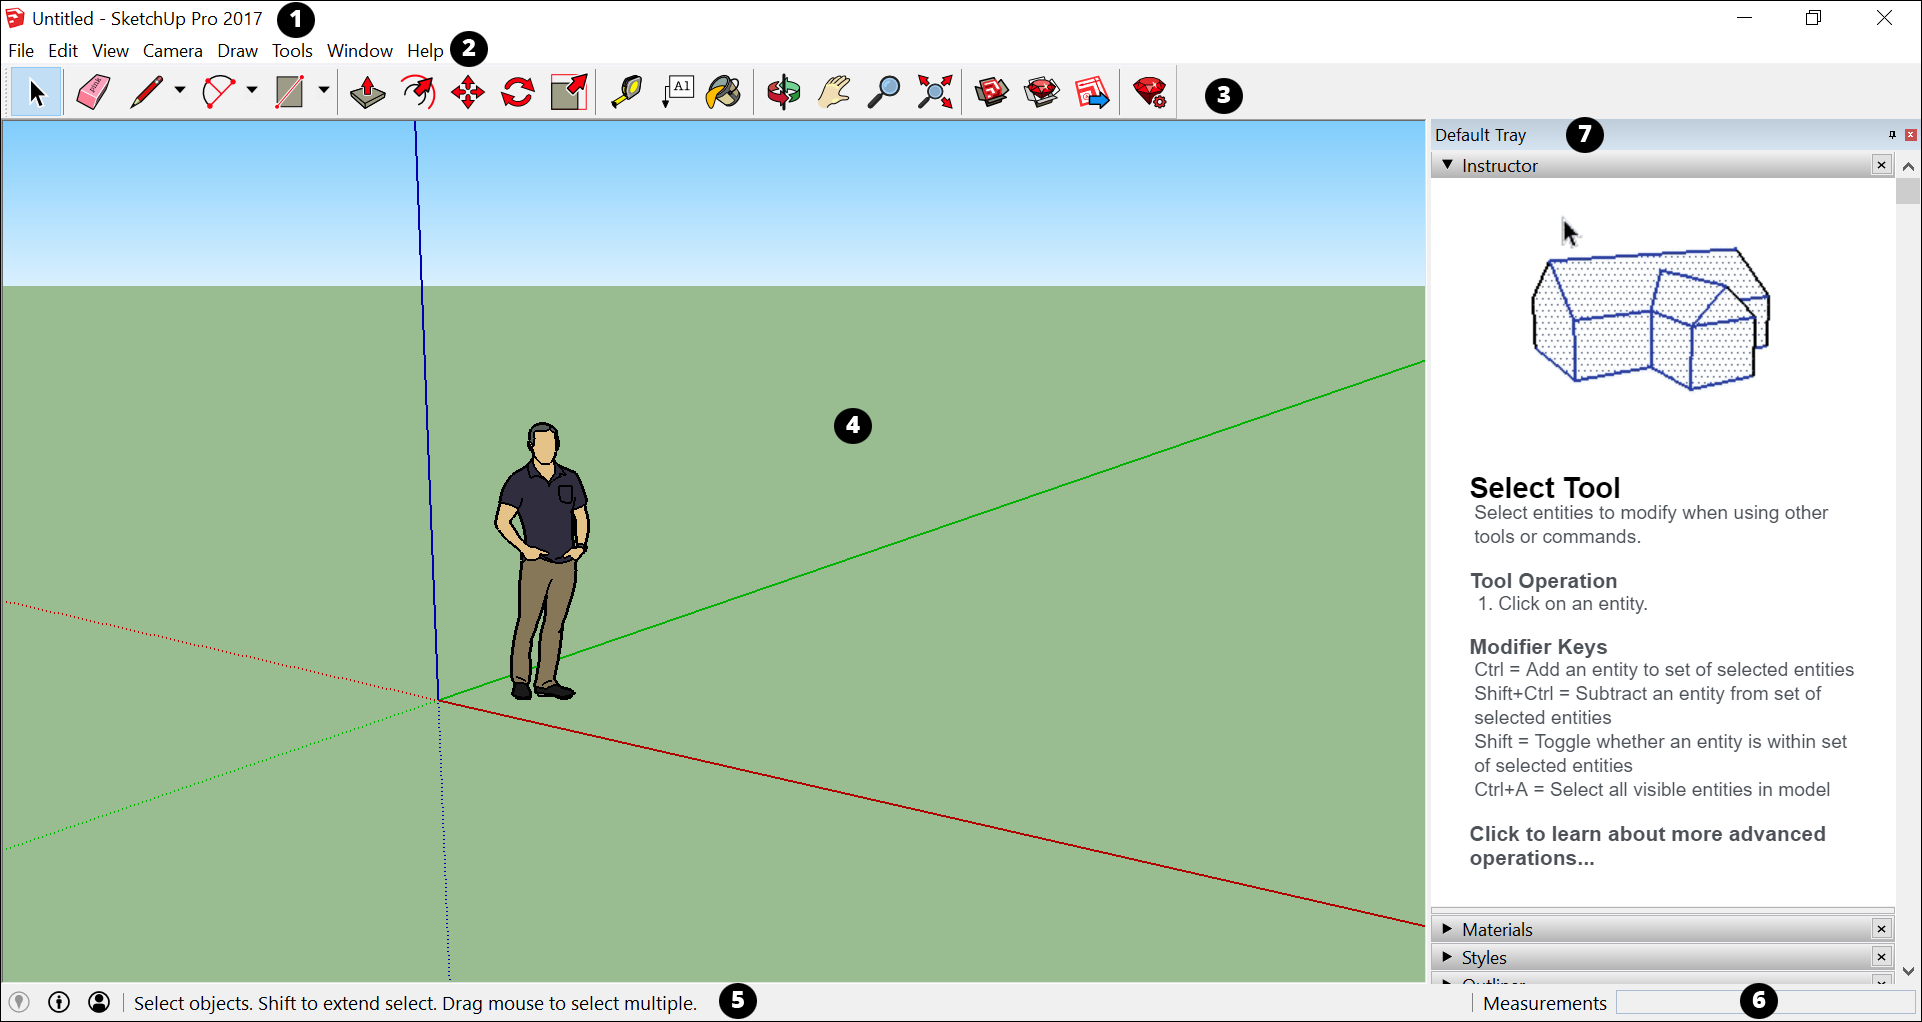
\includegraphics[scale=0.23]{sketchUp}
\\Figure 6: SketchUp UI
\end{center}
\heading{SweetHome3d}SweetHome3d mainly focuses on generating 3D model by drawing 2D floor plan in provided editor simultaneously.If user wants to generate 3D model by importing floor plan image then manual work of tracing and refining an image is required. So, a lot of time is required in doing so.
\begin{center}
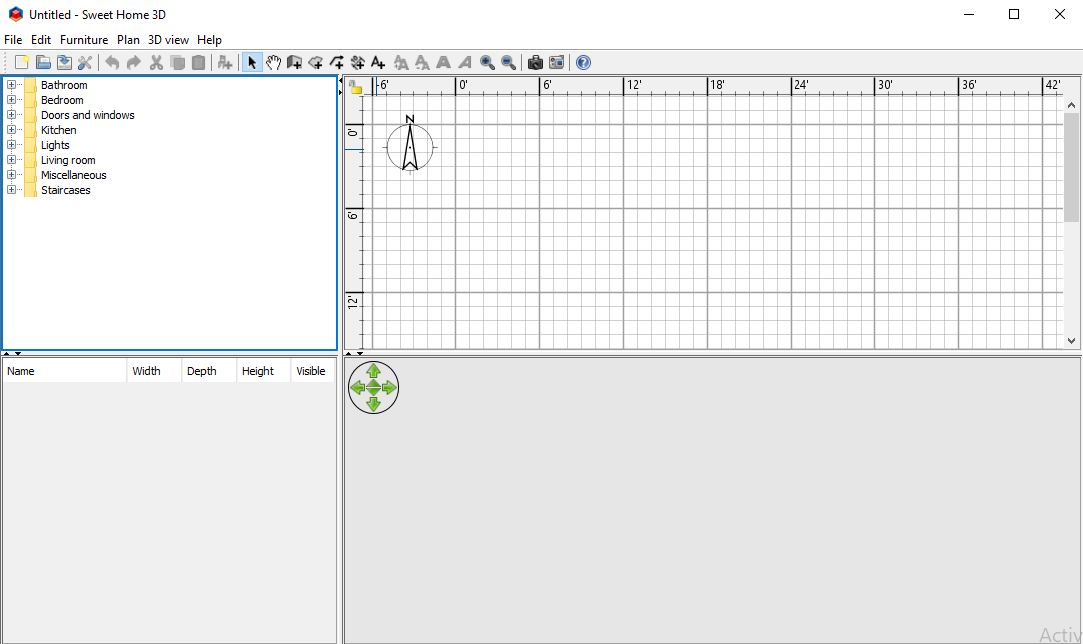
\includegraphics[scale=0.54]{sweetHome}
Figure 7: SweetHome3D UI
\end{center}

\heading{Blender}
Blender is a big platform for modeling, animation, simulation, and game creation. It is very difficult to use because of 100\% customizable interface. It is suitable only for technical users. It requires a lot of effort and time to learn how to use Blender. It allows users to draw 2D floor plan and generate 3D model after a lot of manual work. So, it is not suitable for non-technical users.
\begin{center}
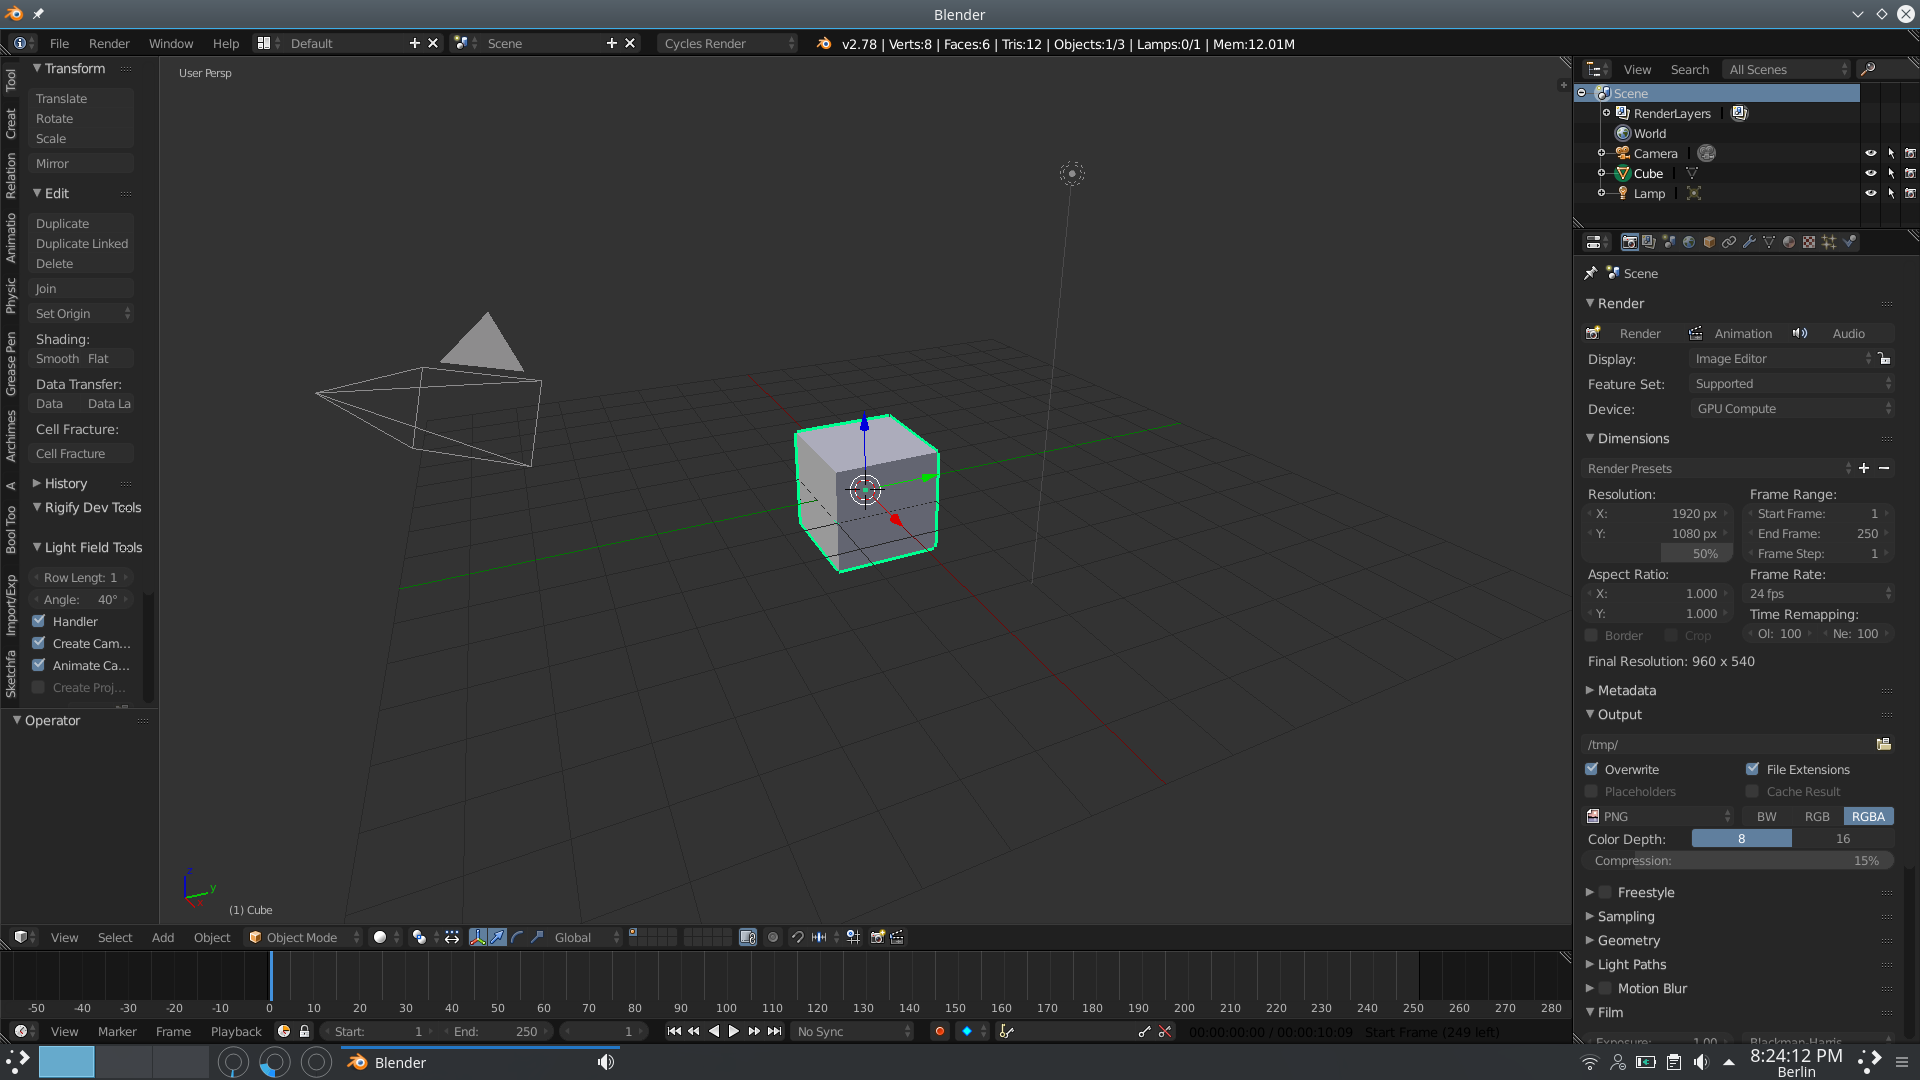
\includegraphics[scale=0.33]{blender}
Figure 8: Blender UI
\end{center}
\heading{FreeCAD Software}
We can create best 3D models through FreeCAD but the problem is again less automation and more manual work is required. Time taking process is required to know how to run the software and also training of the staff is required which will work on it. So, this software is not suitable for normal user.
\\
\begin{center}
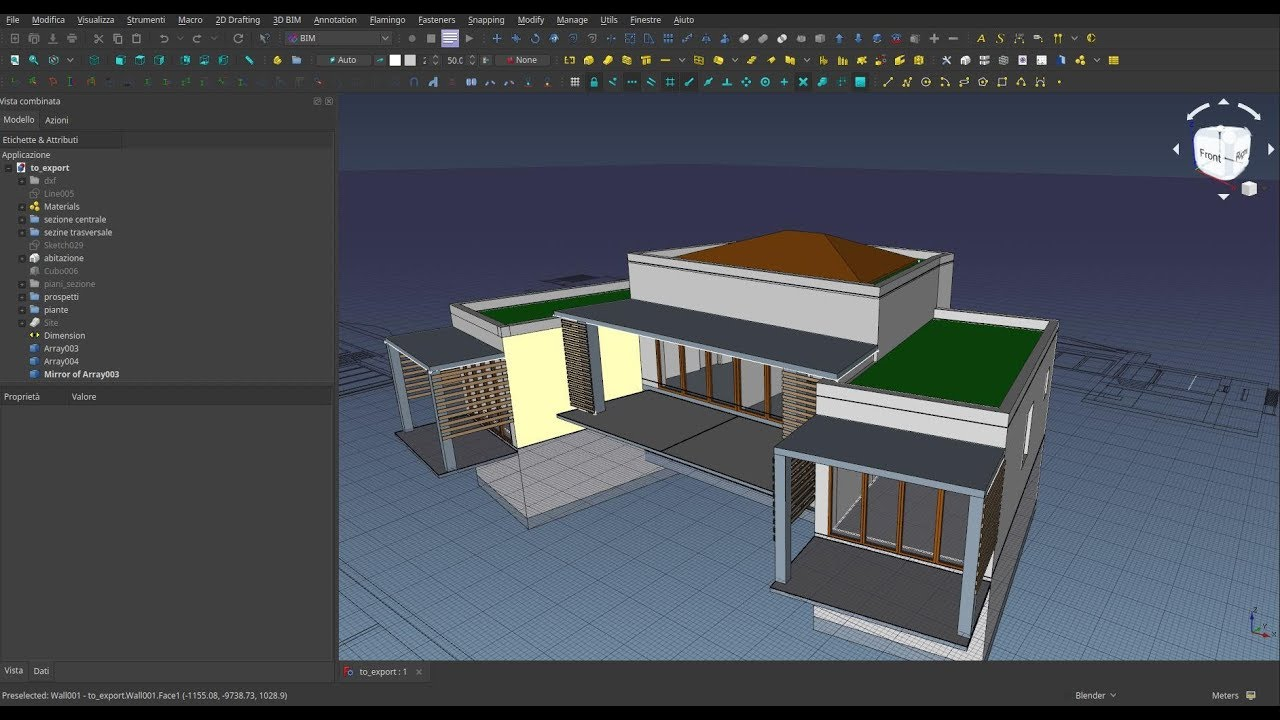
\includegraphics[scale=0.35]{freeCad}
Figure 9: FreeCAD UI
\end{center}
               
\heading{SolidWorks}
SolidWorks mainly focuses on creating 3D models of all types. It does not specifically focus on 3D model of rooms. Although this software is relatively easy to use in comparison to other such softwares but main drawback is its pricing.  Also, it is not suitable software for interior design of home.\cite{freecad}\\
\begin{center}
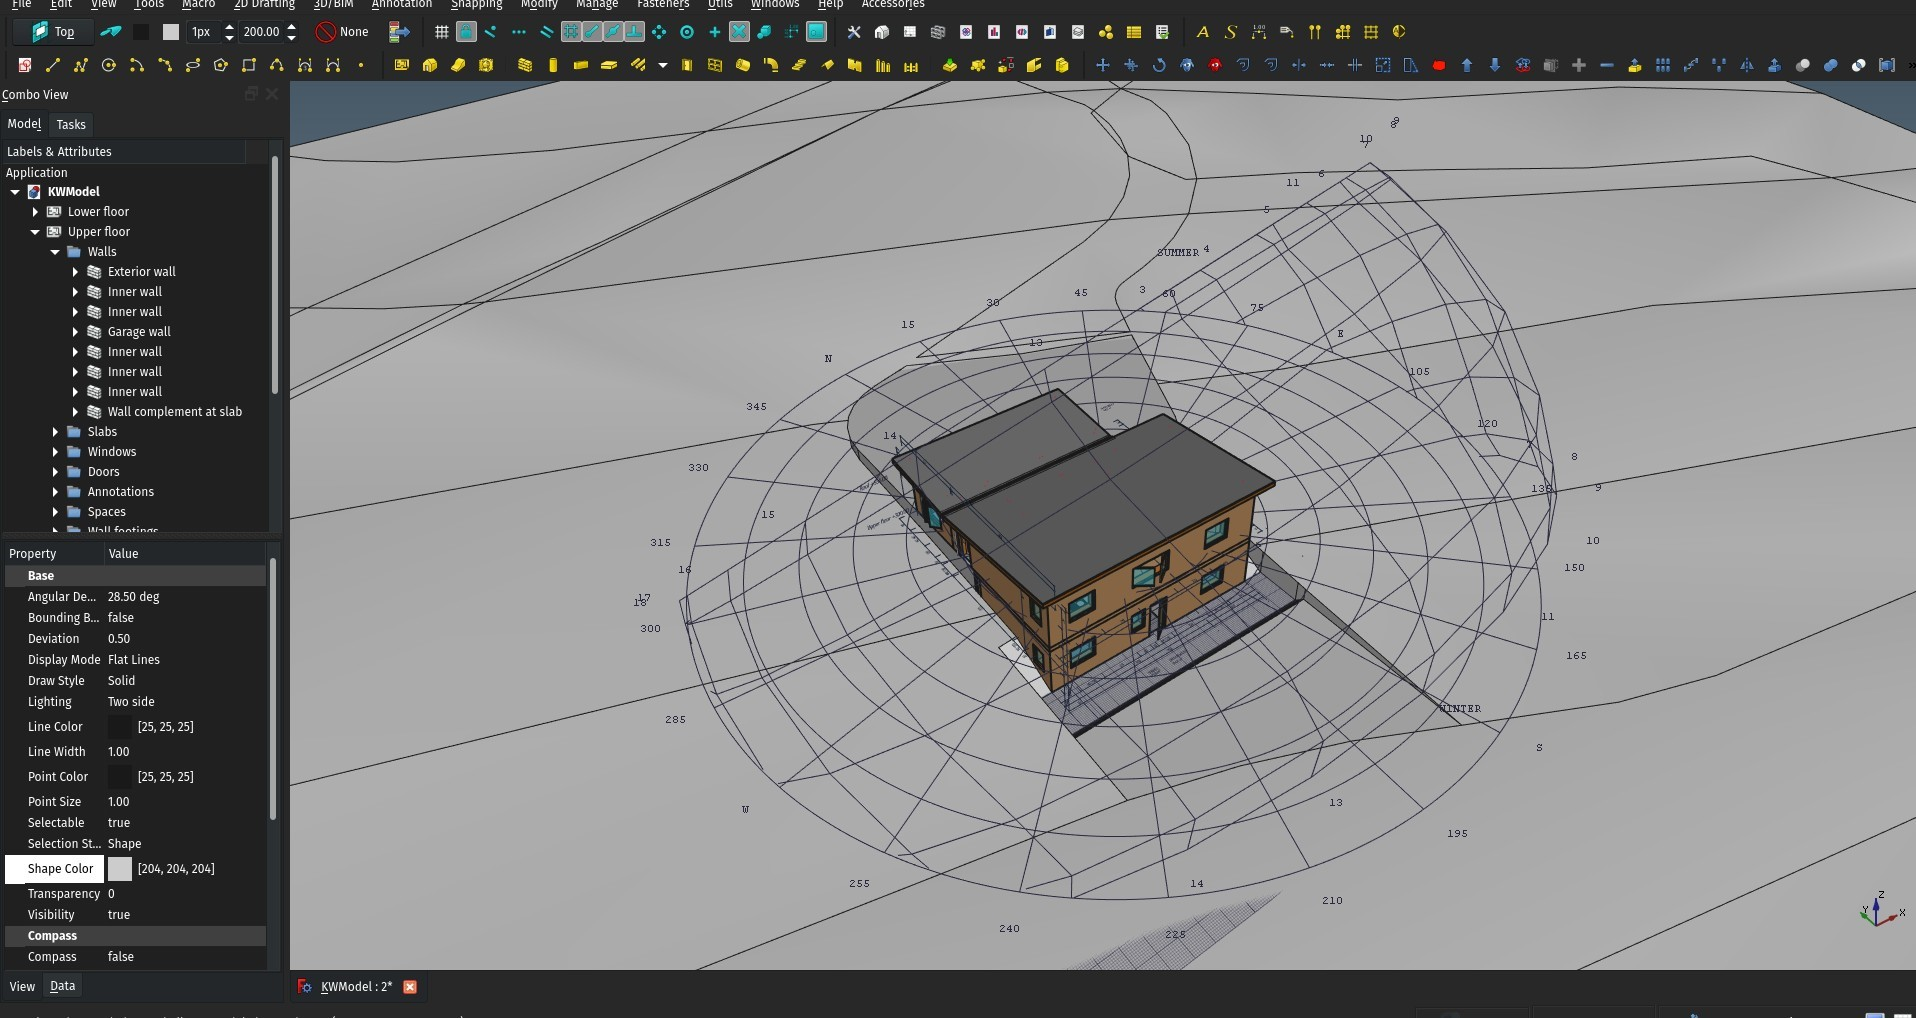
\includegraphics[scale=0.3]{SolidWorks}
\\Figure 10: SolidWorks UI
\end{center}

\section{Problem Statement}
When anyone plans to construct a new flat/house and can only see its floor plan. So it’s hard for anyone to imagine the actual environment by just seeing 2-D floor plan. So, our system will enable the users to see this 2-D floor plan into 3-D and generate 3D model efficiently in less time and effort which existing systems unable to do. Sometimes users also get curious how to design the interior of house. So, this system will also enable users to modify or add furniture in 3-D generated model.
\section{Proposed System}
The application assists users to get their desired 3D model of 2D floor plan in minimum time and price. This also helps users to make decision before the construction of their own houses rather they follow a unrealistic house plan and lose their money, effort and time. This application can be undertaken by architects or common users and anyone who wants his house according to his own desire by having this app from the online stores.
\\
Our project emphasizes on the generation of 3d models from images of 2D floor plans. The project is somehow unique because it focuses on the making of 3d models by importing images of 2D floor plans which is missing in other softwares. Other softwares main concern is to create 3d model from drawn 2d plan and it will be the innovation in our project. Here are functional requirements:
\heading{Import of 2-D floor plan}
User will able to import 2-D floor plan in image format. User can create this floor plan by using Microsoft Office Visio or any other such software.
\heading{Generation of 3-D model}
After clicking on Generate 3-D model button, corresponding 3-D model would be generated.
\heading{Modifications in 3-D model}
User will able to change the texture of walls, height of walls and also modify the walls color by changing the paint color of walls.
\heading{Add  furniture in 3-D model}
User will able to choose any furniture from the list provided (i.e. table, chair and couch etc) and drag at any location in the room.
\heading{Different viewpoints of 3-D model}
User will be able to have different viewpoints of 3-D model i.e. top view, front view and side view. User will also have viewpoint of walk through the 3-D model.

\begin{center}
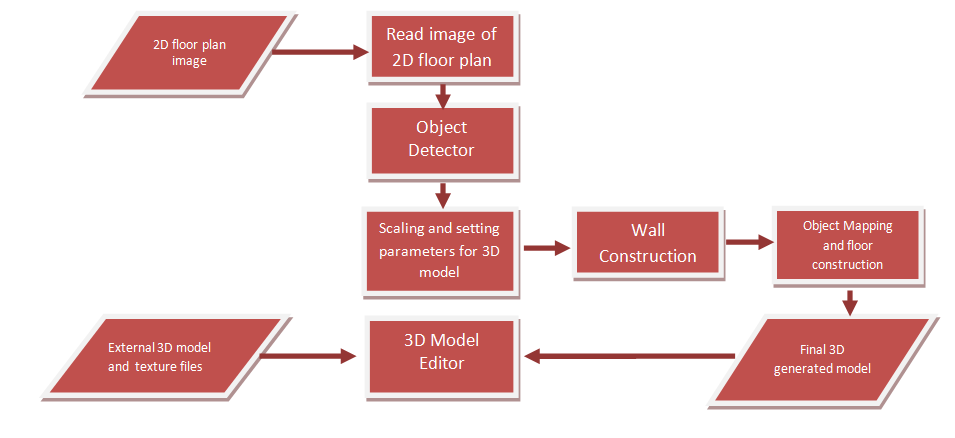
\includegraphics[scale=0.7]{diagram}
\\Figure 11: Proposed system architecture
\end{center}

\section{Feasibility Study}


\subsection{Technical feasibility}
For the development of proposed system, we will use latest technologies. We need any 3D graphics API for the purpose of rendering of 3D models. We can use OpenGL, Irrlicht3D or Direct3D but we choose unity3D. The reason is that OpenGL and Direct3D are low-level APIs which mean we need extremely tough graphical programming for rendering 3D models. Another reason is there were lots of APIs that are built on the top of OpenGL or Direct3D which are relatively easy to use. We can use Irrlicht3D\cite{Irrlicht} but Irrlich3D is neither a latest technology nor it is easy to use.So, finally we choose unity3D graphical engine because it is a latest technology and technically feasible, also it has user-friendly environment for developing applications. Programming language will be C\#. For image recognition and image processing techniques we will use Python 3.6. So, the project’s development is practicable and technically feasible.\cite{TechFeas}\\
\subsection{Operational feasibility}
Operational feasibility means whether a proposed system is to be feasible at operational level. For this purpose, we conduct a market survey in which we ask many questions from common users, architects, home planners and interior designers. 69.7\% people think that their home is not according to what they have imagined at the time of constructing house(see Figure 13). 87.9\% people like to do interior designing of their home on our software to see how it looks before actually doing in real environment(see Figure 14). 51.5\% people use already existing such systems but they don’t like these systems because of hard to use and time taking steps required to generate 3D model(see Figure 15). The proposed system is generate efficiently 3D model on just a button click.
\\
\\
We also conduct survey for architects, home planners and real estate seller agents. 77.3\% people think that they face difficulty in satisfying the customer with their floor plan designs(see Figure 16). 85.7\% people think that the existing systems are not easy to use(see Figure 17). 71.4\% people that existing systems are not cost effective because these softwares are not free(see Figure 18). 90.9\% people are willing to use our proposed system because our proposed system automatically generate 3D model instead of make the 3D model after a lot of manual steps(see Figure 19). 
This study shows that our proposed system is highly operational feasible. There are a lot of drawbacks in existing systems. People want to generate 3D model in less time and with ease. Our proposed system will bring new ideas for efficient sales promotion. Architects and home planners use our proposed system in order to win customer satisfaction. Customer gets their desired dream home exactly according to their imagination. People want to see interior designing of their home according to their imagination without wasting extra money. So, our system is highly acceptable at operational level.
\begin{center}
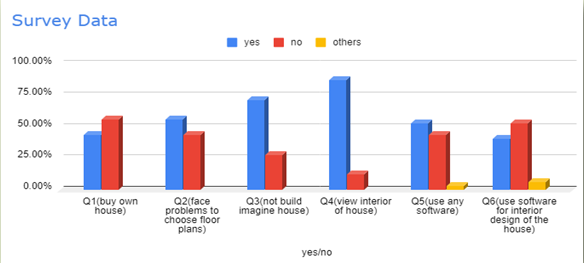
\includegraphics[scale=0.9]{surveydata}
\\Figure 12: Survey reviews
\end{center}


\begin{center}
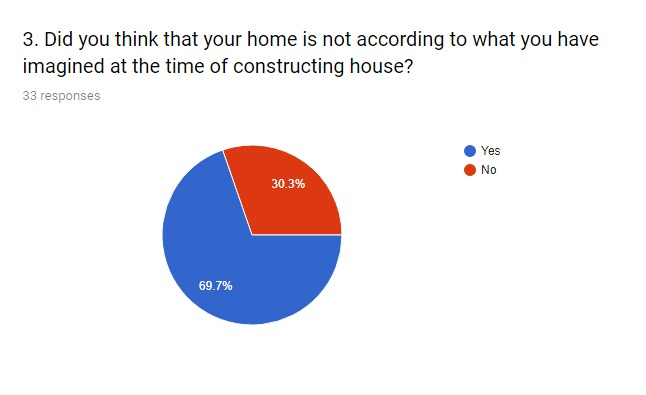
\includegraphics[scale=0.7]{graph3}
\\Figure 13: Not desired house
\end{center}

\begin{center}
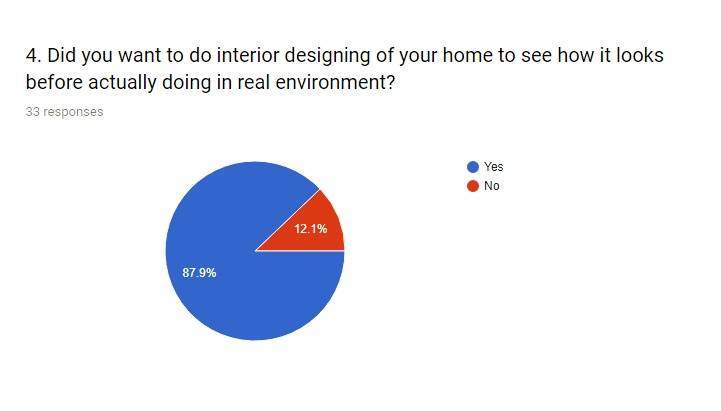
\includegraphics[scale=0.7]{graph4}
\\Figure 14: Interior designing of 3D model
\end{center}

\begin{center}
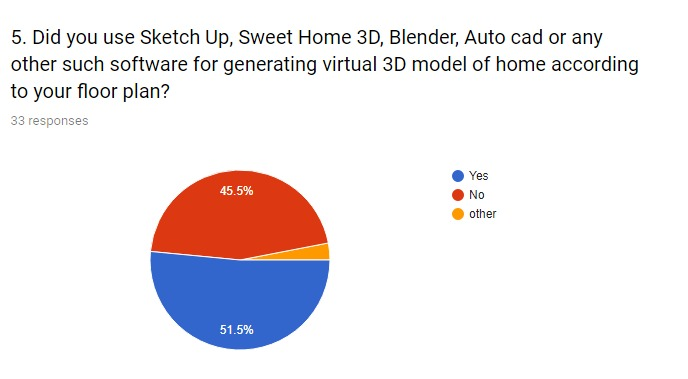
\includegraphics[scale=0.7]{graph5}
\\Figure 15: Use existing systems
\end{center}

\begin{center}
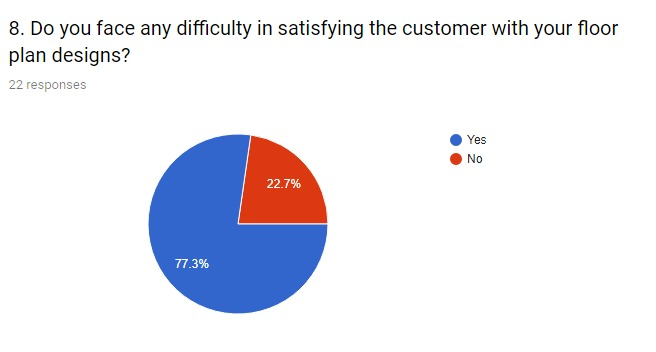
\includegraphics[scale=0.7]{graph8}
\\Figure 16: For architects and home planners
\end{center}

\begin{center}
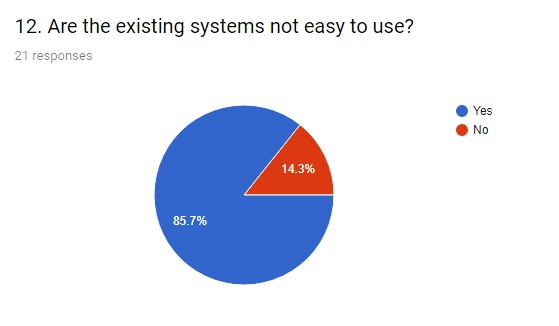
\includegraphics[scale=0.8]{graph12}
\\Figure 17: Not easy to use
\label{fig:five}
\end{center}

\begin{center}
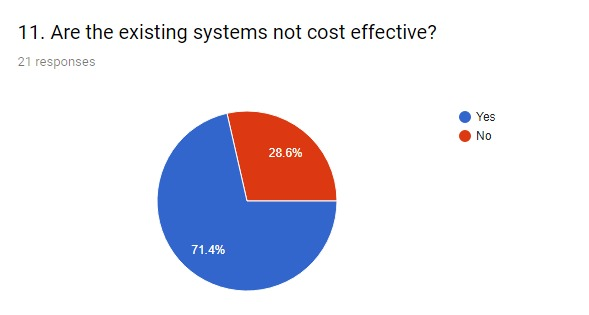
\includegraphics[scale=0.7]{graph11}
\\Figure 18: Not cost effective
\end{center}

\begin{center}
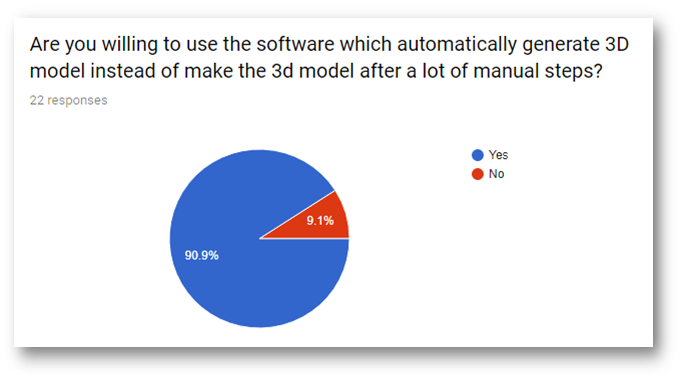
\includegraphics[scale=0.6]{lastgraph}
\\Figure 19: Willing to use our proposed system
\end{center}
 

\subsection{Economical feasibility}

Economical feasibility means whether a project is economically feasible by analyzing the cost required for developing and using this project. There are more than 1 billion PCs/Laptops in use in the world. The number of PC/Laptop users increases day by day. So, this unity based desktop application is feasible for all the users because only existing computer and internet is required for installing the application and if floor plan is in hard form, so for the purpose of capturing  the floor plan only camera is required which almost everyone already have. We built this application by using free and open-source softwares, so no cost is required for developing this application. Only cost involving factor is just having a computer which almost everyone already have. User must know the name of the application and have internet connectivity for the purpose of installing this application. So, this project is highly economical feasible.\cite{econFeas}\\

\section{System Requirements}
\subsection{Hardware Requirements}
\heading{Hardware requirements for Users}
Users just need a laptop/PC in which our application is installed.
\heading{Hardware requirements for Development}
\begin{center}
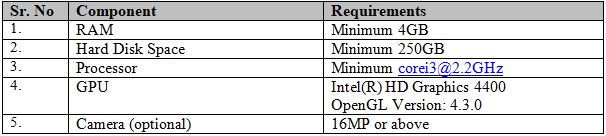
\includegraphics[scale=0.8]{table2}
\\Figure 20: Hardware Requirements
\end{center}
\subsection{Software Requirements}
\heading{Software Requirements for Users}
Users just need a Laptop/PC with Windows Operating System installed.
\heading{Software Requirements for Development}
\begin{center}
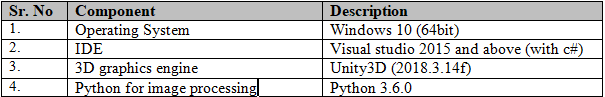
\includegraphics[scale=0.8]{table1}
\\Figure 21: Software Requirements
\end{center}

\section{Limitations and challenges in implementation of project}

\heading{Selection of Software and 3D graphic tools}
We faced a big challenge in selecting a right software and implementing language because simple Visual Studio does not allow to create 3D models, it combines with Unity or some other 3D graphic tool to generate models.
\heading{Compatibility of other programming language with graphic tools}
3D graphic tools i.e. OpenGL and Irrlicht are compatible with C++ but image processing is too much difficult in C++ because we have to generate algorithms at low level. Unity is compatible with C\# and image processing and object detection can be done effectively in python. Because of limitations and incompatibility of programming language with graphic tools, we faced alot of challenges.
\heading{Length of time}
This proposed system is very complex and requires atleast 18 months for completion. But we have to complete this in 7 months which is a big challenge for us.
\heading{Image Processing and recognition}
There are no features in graphics recognition that we can set as reference and recognize a raw data i.e. image. So, for image processing we have to develop recognition algorithms separately for every object detection.
\heading{No background of computer graphics}
We  are facing a lot of challenges regarding 3D graphics. We never used 3D graphics tool or API in past. We searched a lot on latest 3D technologies, use multiple softwares which performs operations in computer graphics i.e. OpenGL, Irrlicht but after much research, we decided to work in Unity graphics scenes with C\# programming language.\cite{unity}\\
\heading{Placing furniture on 3D model according to position and size} 
This is quite difficult to place furniture on 3D model after its construction from 2D floor plan , because it requires co-ordinates adjustment, position and size  of the accessories. A small divergences from a single point or co-ordinate axis results in a distorted 3D model.\cite{chall}

\pagebreak
\section{References}
\begin{thebibliography}{9}

\bibitem{abc} 
ResearchGate: 3D virtual building,
\url{https://www.researchgate.net/publication/221314258}

 
\bibitem{ImageP} 
Image processing: 2D image floor plan,
\\\texttt{https://stackoverflow.com/questions/29471866/creating-a-3d-map-with-2d-depth-images-in-processing}

\bibitem{research} 
Research paper: 3D model from 2D floor plans,
\url{https://www.researchgate.net/publication/288038928_Automatic_reconstruction_of_3D_building_models_from_scanned_2D_floor_plans}

\bibitem{Projectscope} 
Project Scope: Evaluation of project scope,
\url{https://www.brighthubpm.com/project-planning/57950-example-and-evaluation-of-project-scope-statements/}

\bibitem{TechFeas} 
Technical Feasibility,
\url{https://www.brighthubpm.com/project-planning/57950-example-and-evaluation-of-project-scope-statements/}

\bibitem{econFeas} 
Economic Feasibility,
\url{https://www.quora.com/What-does-economic-feasibility-mean}

\bibitem{sketchup} 
Existing System: SketchUp,
\url{https://www.sketchup.com/}

\bibitem{unity} 
3D game engine: Unity3D,
\url{https://unity.com/}


\bibitem{freecad} 
FreeCAD: Pros and Cons,
\url{http://d32l.com/blog/pros-and-cons-of-free-cad-services/}

\bibitem{Irrlicht} 
3D graphics engine: Irrlicht,
\url{http://irrlicht.sourceforge.net/}

\bibitem{limitation} 
Limitation: 3D modelling limitations,
\url{https://search.yahoo.com/yhs/search?hspart=Lkry&hsimp=yhs-newtab&publisherid=55334&type=YHS_VC_55334&p=limitations+doing+3d+project&param1}

\bibitem{chall} 
Challenges: Challenges in project,
\url{https://www.nap.edu/read/22121/chapter/7#33}
\end{thebibliography}
\end{document}